\section{Reproduction of toy experiments}
\label{sec:repr-of-toy}


The first experiment tests whether perturbing the data with small Gaussian noise $\mathcal{N}(0, 0.0001)$ addresses the problem with the manifold hypothesis and facilitates learning. %(implying that the score was not defined before adding noise). %, implicitly meaning the score is defined where it otherwise would not be because of the manifold hypothesis. 
As in \citep{ncsn-paper}, we trained a ResNet encoder-decoder (\autoref{sec:architecture}) on CIFAR-10 with SSM loss for 50,000 iterations (\autoref{fig:toy1}). While we do not get exactly the same magnitude or behaviour of the loss curves as in \cite{ncsn-paper}, we can confirm that the model only converges with perturbed data.% We have included the loss curves in . 

\begin{figure}[h]
  \centering
  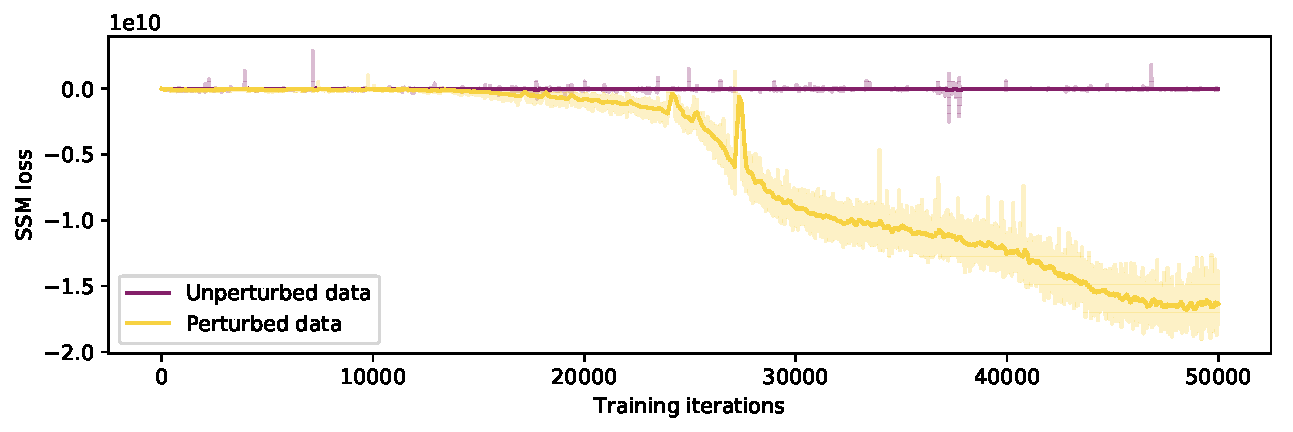
\includegraphics[width=0.83\linewidth]{figures/toy/loss_toy.pdf}
     \caption{Loss curves for score networks trained on
     CIFAR-10 before and after perturbing the data.}
     \label{fig:toy1}
     \vspace{-3mm}
\end{figure}

In the second experiment we compared analytically computed scores (\autoref{fig:anal-grad}) with those estimated by an MLP (\autoref{sec:architecture}) trained with SSM loss for 10,000 iterations (\autoref{fig:est-grad}) for a GMM with $p(\mathbf{x}) = 0.2\ \mathcal{N}\left((-5, -5), \mathbf{I}\right) + 0.8\ \mathcal{N}\left((5, 5), \mathbf{I}\right)$ with near-zero density between the components. The plots look similar to those from the original paper. We can see that scores estimation is accurate in high-density regions around the modes, but fails in low-density ones, as expected.
% \vspace{-2mm}

\begin{figure}[H]
  \centering
     \subfloat[Density of the data]{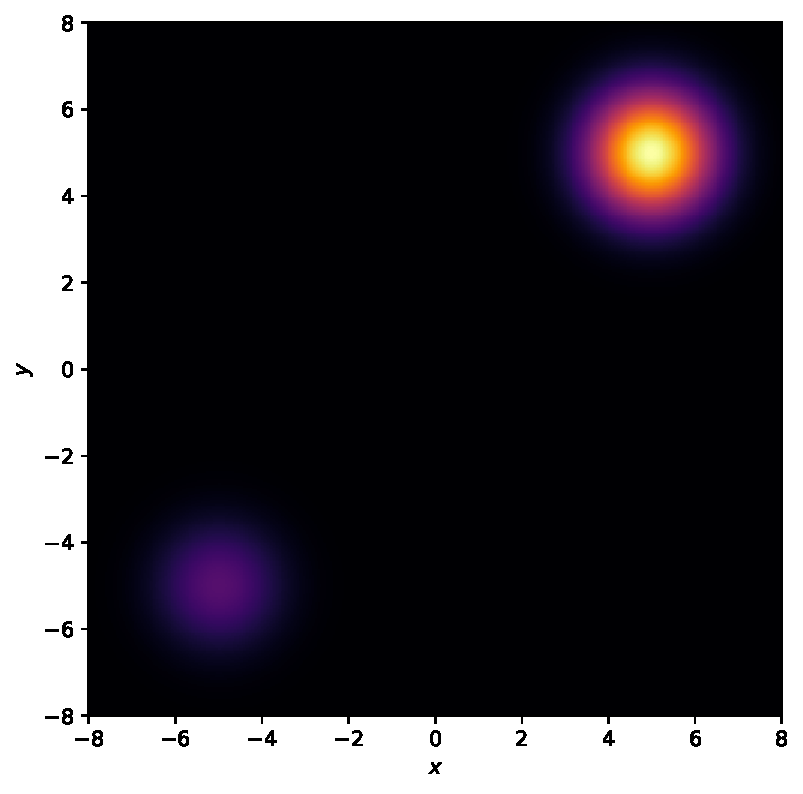
\includegraphics[scale=0.26]{figures/toy/density.pdf}\label{fig:density}}
     \subfloat[True score]{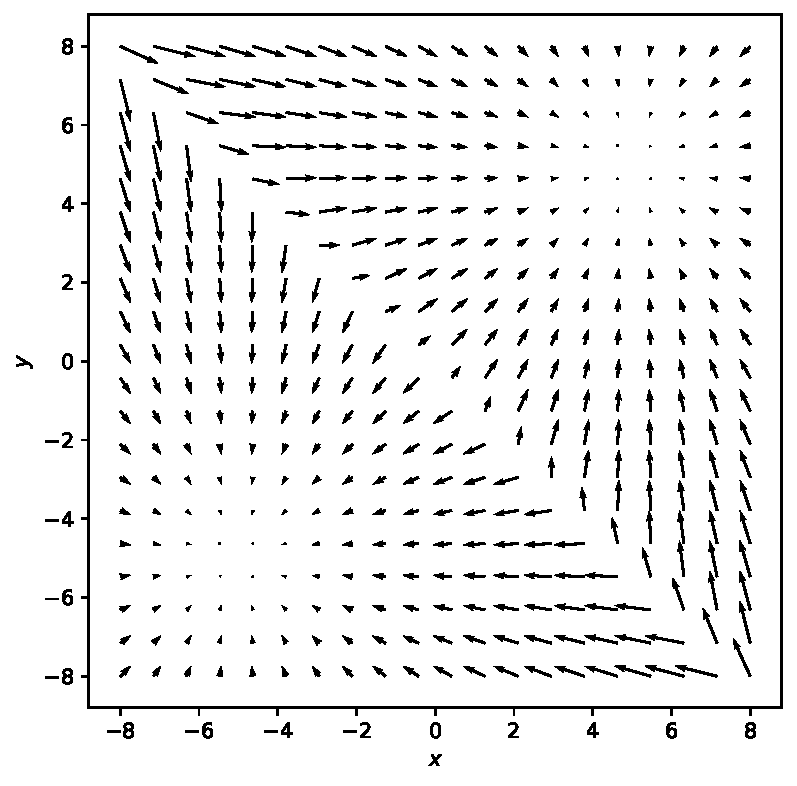
\includegraphics[scale=0.26]{figures/toy/grad_analytic.pdf}\label{fig:anal-grad}}
     \subfloat[Estimated score]{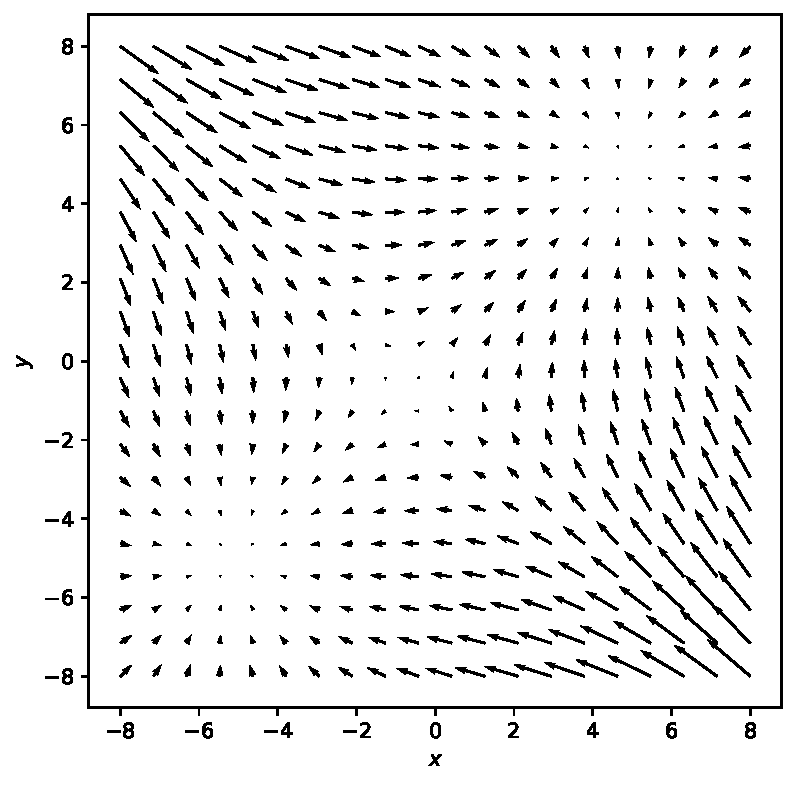
\includegraphics[scale=0.26]{figures/toy/grad-est.pdf}\label{fig:est-grad}}
     \caption{Effect of low-density regions on score estimation.}
     \label{fig:toy2}
     \vspace{-3mm}
\end{figure}

% \subsection{Sampling with Langevin dynamics}
% \label{sec:toy-sampling}

Finally, we attempted to reproduce Figure 3 from the original paper to show the effect of low-density regions on sampling using Langevin dynamics with and without annealing from the GMM from the previous experiment. Here we used the true scores computed analytically. \citet{ncsn-paper} claim that they used a geometric sequence of 10 noise levels $\sigma$ between 10 to 0.1, $T=100$ and $\epsilon=0.1$. However, with this setup, we failed to reproduce the plot (no samples were obtained because of numerical overflow).\footnote{We also confirmed that running the authors' code with these parameters gave the same results.} When consulting with the authors' code, we found that unlike what was reported in \citep{ncsn-paper}, a geometric sequence between 20 and $e^{0.1}$ was used. With these values, we indeed obtained a very similar plot (\autoref{fig:samp-anneal}) to what was reported in the paper.
%\vspace{-2mm}

\begin{figure}[h!]
  \centering
     \subfloat[Exact samples]{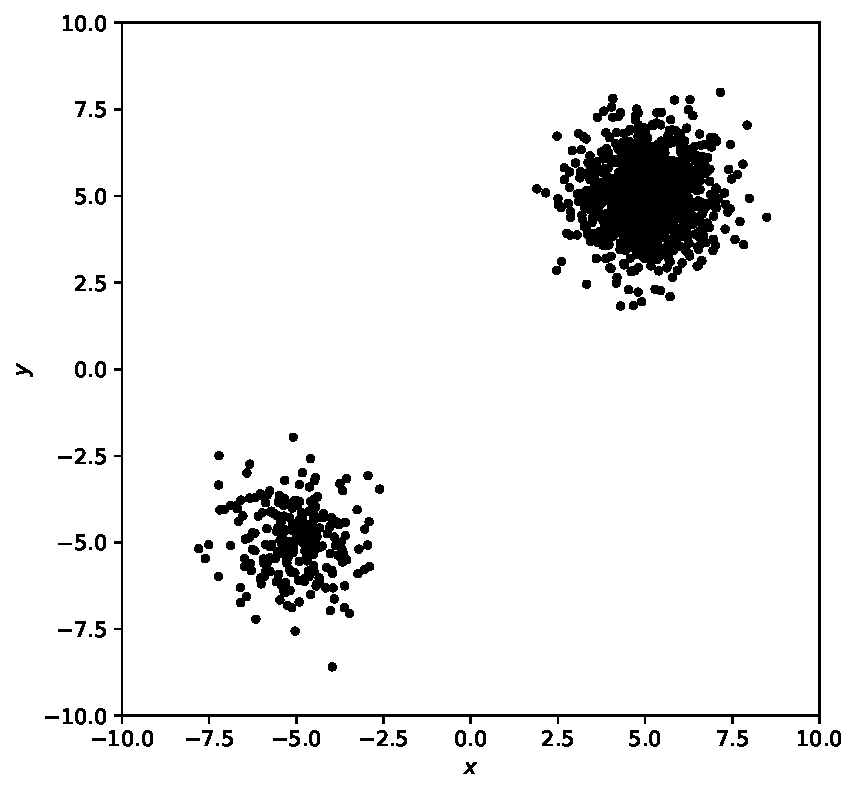
\includegraphics[scale=0.26]{figures/toy/real_samples.pdf}\label{fig:samp}}
     \subfloat[Samples without annealing]{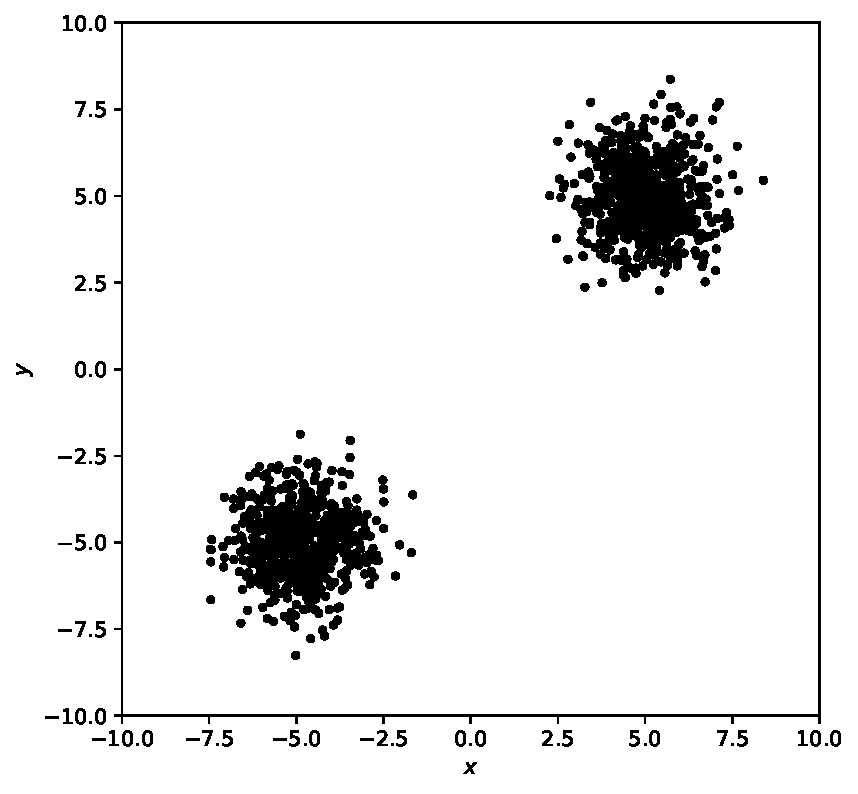
\includegraphics[scale=0.26]{figures/toy/samples_langevin.pdf}\label{fig:samp-langevin}}
     \subfloat[Samples with annealing]{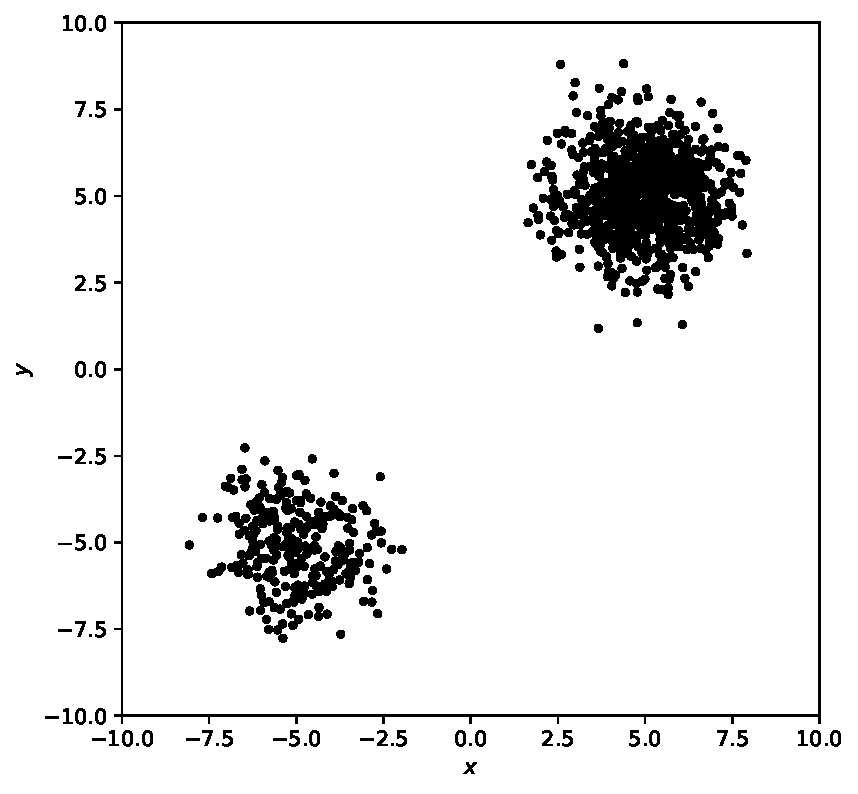
\includegraphics[scale=0.26]{figures/toy/samples_annealed_langevin.pdf}\label{fig:samp-anneal}}
     \caption{Effect of low-density regions on sampling with Langevin dynamics.}
     \label{fig:toy3}
    %  \vspace{-2mm}
\end{figure}

We reason that the reported hyperparameters fail due to step size $\epsilon(\sigma_1 / \sigma_L)^2$, which becomes relatively large when $\epsilon$ and $\sigma_1$ are large or $\sigma_L$ is small. The authors avoid the issue by increasing $\sigma_L$.\footnote{This could be by mistake as the logarithm is applied to $\sigma_1$ but not to $\sigma_L$ when constructing the sequence.} However, this goes against the idea of annealed Langevin dynamics, which is to converge to a distribution which is almost indistinguishable from the true one (i.e. having small $\sigma_L$ is desirable). Therefore we decided to experiment with decreasing $\epsilon$ instead. We include the results in \autoref{fig:eps} in the Appendix. Even with extensive fine-tuning of $\epsilon$ we did not manage to get visually satisfying results, so it is clear that the algorithm is very sensitive to the choice of this hyperparameter. We suggest a goodness-of-fit or a comparison of likelihoods as the future work to quantitatively assess the similarity of distributions.